\documentclass[SDSUThesis.tex]{subfiles} 
\begin{document}

\section{FUTURE WORK}

    Due to the number of issues with surveys.  One area of future work would be indentifying
    a general set of questions that would best fit CRI.  This set would have to include
    the best number of questions, order of questions and wording of questions.  Therefore,
    any new organization would not have to determine their own survey, but rather just use the
    predetermined set of questions.  It would even be advantageous to build a software system to
    handle the survey distribution and collection.  Ideally, the results would automatically be
    inserted into the appropriate database tables for CRI scoring. 
    
    As shown in Table \ref{tab:bsc}, CRI is currently not addressing 2 
    characteristics of the balanced scorecard.  If the SDO does not operate 
    on a fixed budget, CRI could be 
    expanded to include another element for financial data. The challenge arises when
    determining how to relate the SDO performance to finances.  The most likely scenario
    would be a method to either select or predicted the expected software sales
    for a month.  Then every month create an CRI element score that reflects
    how much the expected sales were exceeded or missed.  The other missing
    balanced scorecard characteristic is learning and growth.  Those are very difficult
    to quantitatively measure.  In this case some possible data points might be:
    hours of training, number of training courses, number of employees receiving
    training, number of promotions, or another measure centered around training
    courses and career growth.  Again, once data exists, the problem becomes finding
    a baseline and measuring with respect to that baseline.

    Another area of future work is the expansion of the SDLC-AE to include
    more artifacts of the SDLC.  The more artifacts and processes that can
    be collected, the deeper the understanding of the SDLC.  
    All of the data collection combined with better software analytics
    could lead to true \textit{data-driven software engineering}. Data-driven
    software engineering is the application of collecting and analyzing historical
    information about software engineering artifacts in order to
    accurately predict the outcomes of software engineering projects. This
    will lead to more informed decisions about software engineering.  Figure
    \ref{fig:sdlc-ae-adv} shows an expansion of the previous SDLC-AE diagram.  
    The new elements are in the unshaded boxes, and they are not exhaustive.
    Data-driven software engineering should 
    not to be confused with data-driven programming, in which the computer code
    describes the data instead of the sequence of opertions \cite{DDP2015}.
    
    \begin{figure}[ht]
    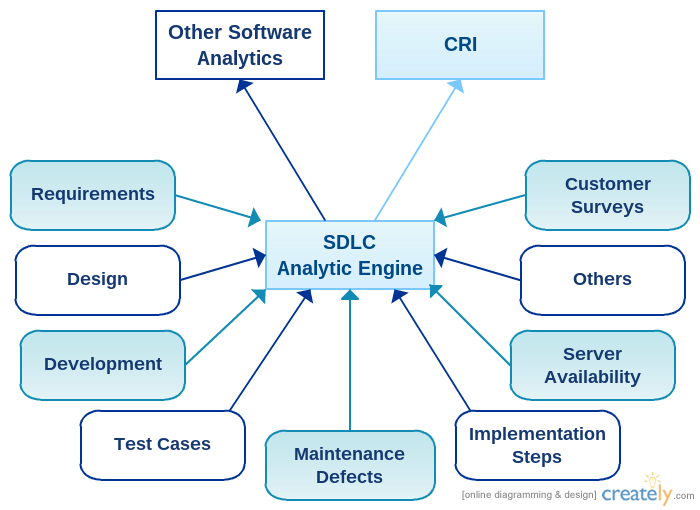
\includegraphics[scale=.75]{images/sdlcae-adv.png}
    \caption{SDLC ANALYTIC ENGINE EXPANSION}
    \label{fig:sdlc-ae-adv}
    \end{figure}
    
    Currently, CRI provides a single method to evaluate past 
    performance, but it does not
    provide any guidance around making more informed future decisions. 
    Some phases are not properly tracked with the initial SDLC-AE and more
    data can be tracked for the existing phases.
    Schedules for each of the individual phases of the SDLC need to be tracked,
    not just the entire project.  Teams need to know how much time is spent
    in design versus testing.  Also, how much time is required to generate
    proper test cases?  These are just a couple of examples of expansions
    to the SDLC-AE.  These and other advancements could lead to greater
    insights about SDLC phases that are struggling and need improvement.
    The SDLC-AE could be expanded to have predictive capabilities.


% new section
\section{CONCLUSION}

There are many metrics that can be used to evaluate a Software Development Organization (SDO). 
Knowing which metrics to use and what they all mean can be a daunting task.  CRI is a
proposed solution to the difficulty of measuring an SDO.

Upon completion, this work shall identify:
\begin{itemize}
    \item Define \textbf{What} characteristics should be measured for an SDO
    \item Define \textbf{How} to measure those characteristics
    \item Map the relationship or lack of relationship with a Balanced Scorecard
    \item Create a Framework to store the necessary data for CRI
    \item Outline a Process to generate the CRI score
    \item Provide an example CRI score with real data
\end{itemize}

An entire software development organization (SDO) needs to be measured and analyzed properly, not just the development portion. This document has provided an overview of what indicators need to be measured for an SDO, and how those indicators can be combined to form a single number indicating the performance score of a software development organization.  Also, a framework to store this data was discussed.

\end{document}